\documentclass{article}

\usepackage[persian, group]{hw}
\usepackage{mips}
\title{تشخیص‌دهنده لبه}
\semester{تابستان ۱۴۰۱}
\course{پردازش چند‌هسته‌ای - پروژه پایانی}
\teacher{دکتر هاجر فلاحتی}
\usepackage{textcomp}
\usepackage{pgfplots}
\pgfplotsset{compat=1.16}

\usepackage{hyperref}
\addauth{فاطمه خاشعی}{fatt3me@gmail.com}{97105899}
\addauth{علی حاتمی تاجیک}{a.hatam008@gmail.com}{98101385}

% Define a custom color
\definecolor{codegreen}{rgb}{0,0.6,0}
\definecolor{codegray}{rgb}{0.5,0.5,0.5}
\definecolor{codepurple}{rgb}{0.58,0,0.82}
\definecolor{backcolour}{rgb}{0.95,0.95,0.92}

% Define a custom style
\lstdefinestyle{myStyle}{
    backgroundcolor=\color{backcolour},   
    commentstyle=\color{codegreen},
    keywordstyle=\color{magenta},
    numberstyle=\tiny\color{codegray},
    stringstyle=\color{codepurple},
    basicstyle=\ttfamily\footnotesize,
    breakatwhitespace=false,         
    breaklines=true,                 
    keepspaces=true,                 
    numbers=left,       
    numbersep=5pt,                  
    showspaces=false,                
    showstringspaces=false,
    showtabs=false,                  
    tabsize=2,
}

% Use \lstset to make myStyle the global default
\lstset{style=myStyle}

\begin{document}
\heading
\header
\allowdisplaybreaks

\tableofcontents
\pagebreak

\section{مقدمه}
در این پروژه سعی شده است که یک تشخیص دهنده‌لبه
\LTRfootnote{Edge Detector}
با استفاده از \lr{Sobel Operator} پیاده‌سازی شود که برروی پردازنده‌های گرافیکی شرکت
\lr{Nvidia} (پلتفرم \lr{CUDA}) اجرا شود.
برای بهبود زمان اجرای برنامه از تکنیک‌هایی برای بالابردن بهره‌وری استفاده شده است و همچنین
برای رابط کاربری بهتر از واسط کاربری گرافیکی استفاده‌ شده است.
شمایل نهایی در شکل \ref{fig:final} آمده است.

\begin{figure}
	\centering
	\includegraphics[scale=0.4]{./resources/final.jpg}
	\caption{شمایل نهایی برنامه}
	\label{fig:final}
\end{figure}

\section{پیاده‌سازی}
پیاده‌سازی انجام شده با استفاده از الگوریتمی که در 
\textcolor{cyan}{\href{https://en.wikipedia.org/wiki/Sobel_operator}{\lr{WikiPedia}}}
آمده بود پیاده‌سازی ساده این الگوریتم را از کد متلبی که داده شده بود الهام گرفتیم و مطابق با آن الگورتیم را در \lr{C++} پیاده‌سازی کردیم.

\subsection{پیاده‌سازی ساده}
ساده‌ترین پیاده‌سازی که به ذهن می‌رسد، پیاده‌سازی کانلوشون و انجام آن روی عکس و در نهایت گرفتن جذر جمع مجذور دو عدد و اعمال آستانه\LTRfootnote{Threshold} نهایی است. البته برای راحتی در پیاده‌سازی فیلترها به صورتی چیده شده اند که ضرب عضو به عضو آنها کفایت کند (چرخاندن فیلتر پیش از اجرای کرنل انجام گرفته است). در این پیاده‌سازی ساده هر ترد مسئول یک پیکسل از خروجی نهایی است و ۹ ضرب (سایز فیلتر) را انجام داده، نتایج را با یکدیگر جمع می‌کند و نتیجه کانولوشن را به ما می‌دهد. این ضرب‌ها با استفاد ها از دو حلقه حول مرکز فیلتر انجام می‌گیرد.
کد کرنل پیاده‌سازی شده در ادامه آمده است.

\begin{latin}
\begin{lstlisting}[language=C++]
__global__ void sobelCUDA(const uint8_t* image, 
    const int8_t* xKernel, 
    const int8_t* yKernel,
    uint8_t* output, 
    int width, 
    int height, 
    int kernelDim, 
    int threshold)
{
    int i = blockIdx.y * blockDim.y + threadIdx.y;
    int j = blockIdx.x * blockDim.x + threadIdx.x;
    int idx = i * width + j;

    int center = (kernelDim - 1) / 2;
    float S1 = 0, S2 = 0;
    int jshift, ishift;
    int out;

    if (i >= center && j >= center && 
        i < height - center && j < width - center) 
    {
        for (int ii = 0; ii < kernelDim; ii++) {
            for (int jj = 0; jj < kernelDim; jj++) {
                jshift = jj + j - center;
                ishift = ii + i - center;
                S1 += image[ishift * width + jshift] * xKernel[ii * kernelDim + jj];
                S2 += image[ishift * width + jshift] * yKernel[ii * kernelDim + jj];
            }
        }

        out = sqrtf(S1 * S1 + S2 * S2);
        out = out > 255 ? 255 : out;
        output[idx] = out > threshold ? out : 0;
    }
}
\end{lstlisting}
\end{latin}

\subsection{پیاده‌سازی بهینه‌سازی شده}
مشکلی که در کد بالا وجود دارد این است که دسترسی به حافظه‌ای بالا وجود دارد و همینطور با
علم به اینکه قرار است چند ضرب و جمع وجود داشته باشد اما با این حال از حلقه‌های تو در تو
استفاده شده است که باعث می‌شود هم دسترسی به حافظه بیهوده داشته باشیم و هم دستورات مربوط به حلقه بار اضافی برای اجرا باشند. راه حل این است که ما فیلتر‌ها را از پیش داریم و میدانیم که از هر کدام سه ضرب و جمع بیهوده استفاده می‌شوند (چرا که عامل صفر را داریم ضرب می‌کنیم!).
برای همین از این روش استفاده می‌کنیم که فیلتر‌ها را به صورت کد-سخت شده
\LTRfootnote{Hard-Coded}
درون کد کرنل می‌آوریم. با این کار هم دسترسی به حافظه که مربوط به فیلتر‌ها بوده است را کم کرده‌ایم، هم حلقه‌ها را از بین برده‌ایم، هم از صفر بودن عامل‌های فیلتر برای کم کردن تعداد دستورات و هم از معلوم بودن فیلتر برای کم کردن تعداد ضرب‌ها (تبدیل ضرب در ۱ و ۱- به جمع و تفریق) استفاده کرده‌ایم. همچنین از الگوی دسترسی منظمی نیز برای کم‌شدن \lr{miss} در حافظه کش استفاده شده‌ است. در کرنل بهینه‌سازی‌شده از قطعه کد زیر به جای حلقه‌های تو در تو استفاده شده‌ است:
\begin{latin}
\begin{lstlisting}[language=C++]
S1 = image[(i - 1) * width + (j + 1)] - image[(i - 1) * width + (j - 1)] +
	(image[(i + 1) * width + (j + 1)]) - image[(i + 1) * width + (j - 1)] +
    2 * ( image[i * width + (j + 1)] - image[i * width + (j - 1)]);

S2 = image[(i - 1) * width + (j - 1)] + (image[(i - 1) * width + (j + 1)]) +
     2 * (image[(i - 1) * width + j] - image[(i + 1) * width + j])
     - image[(i + 1) * width + (j - 1)] - image[(i + 1) * width + (j + 1)];
\end{lstlisting}
\end{latin}

\subsection{افزودن \lr{Shared Memory}}
در این قسمت برای کم کردن دسترسی به حافظه از \lr{Shared Memory} استفاده می‌کنیم که پیش از عملیات اصلی آن قسمتی از عکس که در اجرای کد اصلی استفاده می‌شود را در حافظه اشتراکی بریزیم. در قسمت \ref{perf}
به این مسئله می‌پردازیم که این کار نه تنها باعث افزایش سرعت نمی‌شود بلکه از سرعت می‌کاهد.
در هر بلوک ۱۰۲۴ ریسه در چیدمان ۳۲ در ۳۲ کار می‌کنند و هر کدام مسئول یک پیکسل از
خروجی هستند که هرکدام به پیکسل‌های اطراف خودشان نیاز دارند که با این حساب در هر
بلوک از داده‌های یک قسمت ۳۴ دز ۳۴ از عکس اصلی استفاده می‌شود. برای این کار ابتدا هر ترد
پیکسل منطبق بر پیکسل خروجی را از ورودی به حافظه اشتراکی می‌آورد. سپس ریسه‌هایی که در لبه‌های
قسمت ۳۲ در ۳۲ عکس اصلی قرار دارند پیکسل‌های مجاور خود که در خارج از محدوده ۳۲ در ۳۲ قرار دارند می‌آورند. شکل \ref{fig:shem} نشان می‌دهد که مسئول خواندن هر پیکسل که در حافظه اشتراکی قرار می‌گیرد
با کدام ترد متناظر است (تنها برای پیکسل‌های کناری در شکل نشان‌داده شده‌اند).

\begin{figure}
	\centering
	\includegraphics[scale=1]{./resources/shem.jpg}
	\caption{خواندن داده‌های لبه}
	\label{fig:shem}
\end{figure}

حافظه اشتراکی به وسیله قطعه کد زیر که پیش از کد اصلی قرار می‌گیرد پر می‌شود:

\begin{latin}
\begin{lstlisting}[language=C++]
    __shared__ uint8_t sdata[34 * 34];
    if (i < height && j < width) {
        // Main data
        sdata[(y + 1) * 34 + x + 1] = image[idx];

        // Fix Boudnries
        if (y == 0 && blockIdx.y != 0) {
            sdata[x + 1] = image[(i - 1) * width + j];
            if (x == 0 && blockIdx.x != 0) {
                sdata[0] = image[(i - 1) * width + (j - 1)];
            }
        }
        if (x == 0 && blockIdx.x != 0) {
            sdata[y34 + 34] = image[(i)*width + j - 1];
            if (y == 31 && i != height - 1) {
                sdata[33 * 34] = image[(i + 1) * width + j - 1];
            }
        }
        if (y == 31 && i != height - 1) {
            sdata[33 * 34 + x + 1] = image[((i + 1) * width + j)];
            if (x == 31 && j != width - 1) {
                sdata[33 * 34 + 33] = image[(i + 1) * width + j + 1];
            }
        }
        if (x == 31 && j != width - 1) {
            sdata[y34 + 34 + 33] = image[i * width + j + 1];
            if (y == 0 && blockIdx.y != 0) {
                sdata[33] = image[(i - 1) * width + j + 1];
            }
        }
    }

    // waits untill shared data is completed
    __syncthreads();
\end{lstlisting}
\end{latin}

حال قطعه کد اصلی به جای اینکه از حافظه داده خود را بردارد از حافظه اشتراکی این کار را انجام می‌دهد.

\subsection{تغییر روشنایی}
برای تغییر روشنایی از یک کرنل ساده استفاده می‌شود که کد آن در ادامه آمده است. پس از افزودن مقدار مورد نظر به هر پیکسل، اگر از باند مربوط به یک پیکسل گذشته بود آنرا به محدوده برمی‌گردانیم.

\begin{latin}
\begin{lstlisting}[language=C++]
__global__ void changeBrightnessCUDA(uint8_t* input, const int width, 
    const int height, const int brightness)
{
    int val;

    int i = blockIdx.y * blockDim.y + threadIdx.y;
    int j = blockIdx.x * blockDim.x + threadIdx.x;
    int idx = i * width + j;

    if (i < height && j < width) {
        val = input[idx] + brightness;
        // Truncate the result (0..255)
        if (val > 255) {
            val = 255;
        }
        else if (val < 0) {
            val = 0;
        }
        input[idx] = val;
    }
}
\end{lstlisting}
\end{latin}


\subsection{پیکربندی اجرای کرنل}
اجرای کرنل‌ها روند کلی زیر را طی می‌کند:
\begin{enumerate}
	\item حافظه عکس اصلی تخصیص داده می‌شود.
	\item عکس در حافظه کپی می‌شود.
	\item کرنل تغییر روشنایی اجرا می‌شود.
	\item صبر می‌شود تا تغییرات صورت بگیرد.
	\item نتیجه به صورت آسنکرون روی استریمی جدا به هاست منتقل می‌شود.
	\item حین جابجایی عکسی که روشنایی آن تغییر کرده است کرنل تشخیص لبه اجرا می‌شود.
	\item نتیجه نهایی به هاست منتثقل می‌شود.
\end{enumerate}

در ادامه کد اجرایی آمده است. البته برای خوانایی گزارش به صورت خلاصه‌ آمده است.

\begin{latin}
\begin{lstlisting}[language=C++]
	dim3 block(BLOCK_DIM, BLOCK_DIM);
	dim3 grid(width/BLOCK_DIM + (width%BLOCK_DIM!=0), 
		height/BLOCK_DIM + (width % BLOCK_DIM != 0));

	cudaMalloc((void**)&dev_input, imageSize);
	cudaMalloc((void**)&dev_edge, imageSize);
	cudaMemcpy(dev_input, input, imageSize, cudaMemcpyHostToDevice);

	changeBrightnessCUDA <<<grid, block, 0, main>>> (dev_input, width, height, brightness);
	cudaGetLastError();
	cudaDeviceSynchronize();

	cudaMemcpyAsync(bright, dev_input, imageSize, cudaMemcpyDeviceToHost, mem);

	sobelOptimizedShCUDA <<<grid, block, 0, main>>> (dev_input, dev_edge, width, height, threshold);
	cudaEventRecord(stop);
	cudaGetLastError();
	cudaDeviceSynchronize();
\end{lstlisting}
\end{latin}

در اینجا با فرستادن غیرهمگام تصویری که روشنایی آن تغییر کرده است، از اورلپ صورت گرفته
را در زمان نهایی ذخیره می‌کنیم و \lr{Thoughput} حافظه را افزایش می‌دهیم.

دلیل نحوه انتخاب این سایز برای بلوک در بخش \ref{perf}  توضیح داده شده است.

\section{بررسی و مقایسه عملکرد}
\label{perf}

در ابتدا به مقایسه علملکرد کرنل‌های متفاوت می‌پردازیم. نتیجه \lr{Benchmark} اجرا شده روی کد‌های مختلف در نمودار شکل \ref{fig:perf} آمده است. (دقت شود که اندازه محور زمان لگاریتمی است). در این شکل به وضوح زمان بهتر اجرا بر روی \lr{GPU} آمده است.
برای این تست از سخت‌افزار زیر استفاده شده است:
\begin{latin}
\begin{itemize}
	\item[CPU] 11th Gen Intel \textregistered Core\texttrademark i7-1165G7 @ 2.80GHz
	\item[GPU] NVIDIA GeForce MX450
\end{itemize}
\end{latin}
\begin{figure}
\centering
\begin{latin}
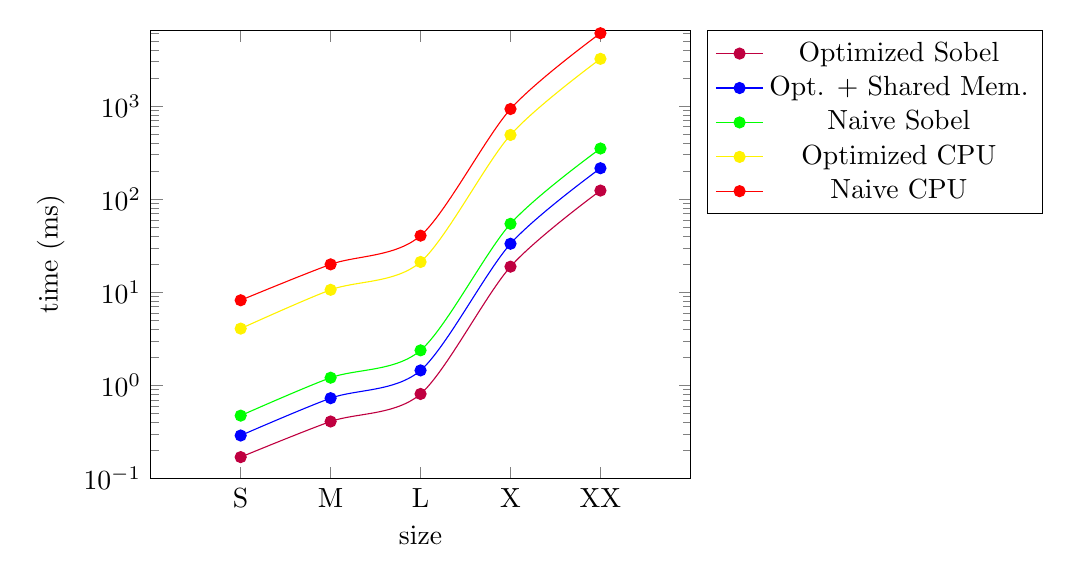
\begin{tikzpicture}
\begin{axis}[
	legend pos=outer north east,
    xlabel=size,
    ylabel=time (ms),
    xmin=0, xmax=60,
    ymin=0.1, ymax=6500,
    ymode=log,
    xtick={10, 20, 30, 40, 50},
    xticklabels={S, M, L, X, XX}
            ]
\addplot[smooth,mark=*,purple] plot coordinates {
    (10,0.17)
    (20,0.41)
    (30,0.81)
    (40,18.84)
    (50,123.60)
};
\addlegendentry{Optimized Sobel}

\addplot[smooth,mark=*,blue] plot coordinates {
    (10,0.29)
    (20,0.73)
    (30,1.45)
    (40,33.18)
    (50,214.72)
};
\addlegendentry{Opt. + Shared Mem.}

\addplot[smooth,mark=*,green] plot coordinates {
    (10,0.474)
    (20,1.21)
    (30,2.38)
    (40,54.366)
    (50,349.62)
};
\addlegendentry{Naive Sobel}

\addplot[smooth,mark=*,yellow] plot coordinates {
    (10,4.074)
    (20,10.63)
    (30,21.159)
    (40,488.90)
    (50,3207.36)
};
\addlegendentry{Optimized CPU}

\addplot[smooth,mark=*,red] plot coordinates {
    (10,8.21)
    (20,19.94)
    (30,40.55)
    (40,927.79)
    (50,6044.46)
};
\addlegendentry{Naive CPU}
\end{axis}
    \end{tikzpicture}
\end{latin}
\caption{نتایج بنچ‌مارک انجام شده روی متدهای مختلف}
\label{fig:perf}
\end{figure}
سایز تصاویر به شرح زیر است:
\begin{latin}
\begin{itemize}
	\item[S] 729 x 480
	
	\item[M] 1166 x 768
	
	\item [L] 1639 x 1080
	
	\item[X] 7881 x 5192
	
	\item[XX] 20000 x 13176
\end{itemize}
\end{latin}
حال به برخی توضیحات می‌پردازیم.

\subsection{دلیل بیشتر بودن زمان هنگام استفاده از حافظه اشتراکی}
پس از اینکه متوجه این مورد شدیم که زمان اجرای هنگامی که از حافظه اشتراکی 
استفاده می‌شود بر خلاف انتظارات بیشتر از حالتی است که تماما از حافظه اصلی
می‌خوانیم با استفاده از نرم‌افزار \lr{Nsight Conpute} به پروفایلینگ
تست انجام شده پرداختیم. پس از بررسی‌های انجام شده به این نتیجه رسیدیم که دلیل بیشتر شدن زمان این موضوع است که در کد \lr{divergant}‌هایی ایجاد شده است که
کارایی را پایین آورده است. همچنین در حالتی که از حافظه اصلی استفاده می‌شود
\lr{Hit Rate} بالایی در کش مرحله اول داریم که باعث می‌شود بدون حافظه اشتراکی
دسترسی به حافظه همانند حالت اشتراکی باشد. در شکل \ref{fig:perf:sh}
و \ref{fig:perf:opt} آنالیزهای مربوط به حافظه آمده است. همچنین آنالیز کلی
صورت گرفته در محل
\verb!./resources/profile.ncu-rep!
موجود است.

\begin{figure}
	\centering
	\includegraphics[scale=0.5]{./resources/perf-opt}
	\caption{آنالیز مموری حالت بدون حافظه اشتراکی}
	\label{fig:perf:opt}
\end{figure}


\begin{figure}
	\centering
	\includegraphics[scale=0.5]{./resources/perf-sh}
	\caption{آنالیز مموری حالت حافظه اشتراکی}
	\label{fig:perf:sh}
\end{figure}


\subsection{دلیل انتخاب سایز بلوک}
با توجه به آنالیزی که روی کد انجام گرفته است، اندازه ۱۰۲۴ برای بلوک مناسب‌ترین
سایز است و چون سر و کارمان با عکسهاست، اندازه ۱۰۲۴ در ۱ می‌تواند پرتی زیادی در ابعداد ایجاد کند برای همین از بلوک‌های مربعی ۳۲ در ۳۲ استفاده کرده‌ایم که کمترین‌ بلوک ممکن در مساحت استفاده شود. در شکل \ref{fig:block} آنالیز تعداد بلوک آمده است.

\begin{figure}
\centering
\includegraphics[width=\textwidth]{./resources/warp}
\caption{آنالیز تعداد بلوک حافظه}
\label{fig:block}
\end{figure}

\section{رابط کاربری گرافیکی}
همانطور که از شکل \ref{fig:final} پیداست، رابط گرافیکی شامل پنج بخشی کلی است:
\begin{itemize}
	\item نمایش ورودی
	
	\item نمایش ورودی تغییر یافته (روشنایی)
	
	\item نمایش خروجی
	
	\item انجام تنظیمات قبل از اجرای الگوریتم
	
	\item آمار مربوط به اجرا
\end{itemize}

تنظیمات قبل از اجرا شامل تنظیمات روشنایی و آستانه می‌شود.
در منوی فایل همچنین باز کردن، ذخیره‌کردن،‌ نمایش بزرگتر تصویر خروجی (زمانی که تصاویر بزرگ باشند، خروجی که نمایش داده می‌شود از دقت بالایی برخوردار نیست) و بستن برنامه است (شکل \ref{fig:file}). هنگام بستن و یا تعویض ورودی اگر تغییرات ذخیره نشد‌ه‌ای وجود داشته باشد از کاربر تاییدی برای ذخیره کردن یا نکردن گرفته می‌شود. برای پیاده‌سازی این رابط کاربری از فریم‌ورک \lr{Qt}
استفاده شده است.

\begin{figure}
	\centering
	\includegraphics[scale=0.8]{./resources/file}
	\caption{منو فایل}
	\label{fig:file}
\end{figure}

\section{جمع‌بندی}
در این پروژه یک تشضخیص‌دهنده لبه برای \lr{CUDA} پیاده‌سازی شده است که دارای ویژگی‌های زیر است:
\begin{itemize}
	\item استفاده از مکانیز‌م‌هایی برای بهینه‌سازی الگوریتم:
	\begin{itemize}
		\item حذف دسترسی حافظه برای فیلتر
		\item حذف کردن حلقه \LTRfootnote{Loop Unrolling}
		\item در نظر نگرفتن عامل‌های صفر
		\item استفاده از الگوی دسترسی به حافظه منظم
		\item راهکاری برای استفاده از حافظه اشتراکی با تداخل بانک صفر (به قصد افزایش سرعت)
		\item استفاده از اندازه بلوک بهینه
		\item استفاده از کپی غیرهمگام برای همپوشانی کار مموری و محاسبات
	\end{itemize}
	\item پشتیبانی از اندازه‌های بزرگ (\lr{8k})
	\item پیاده‌سازی آستانه
	\item پیاده‌سازی \lr{GUI}
\end{itemize}


\end{document}
